\documentclass[10pt,aps,onecolumn,superscriptaddress]{revtex4-2}

\usepackage[T1]{fontenc}
\usepackage[utf8]{inputenc}
\usepackage[english]{babel}

\usepackage{amsfonts,amsbsy,amssymb,amsmath}
\usepackage{graphicx,float}
\usepackage{hyperref}
\hypersetup{
    colorlinks=true,
    linkcolor=blue,
    filecolor=magenta,      
    urlcolor=cyan,
}

\graphicspath{{notebooks/figures/}}

\bibliographystyle{apsrev4-2}

\begin{document}

\title{Chemical Reaction Dynamics on the Cirque Potential Energy Surface}

\author{Broncio Aguilar Sanjuan}
\email{broncio.aguilarsanjuan@bristol.ac.uk}
\affiliation{School of Mathematics, University of Bristol, \\ Fry Building, Woodland Road, Bristol, BS8 1UG, United Kingdom.}

\author{V\'ictor J. Garc\'ia-Garrido}
\email{vjose.garcia@uah.es}
\affiliation{Departamento de F\'isica y Matem\'aticas, Universidad de Alcal\'a, \\ Alcal\'a de Henares, 28871, Spain.}

\author{Francisco Gonz\'alez Montoya}
\email{fg16704@bristol.ac.uk}
\affiliation{School of Mathematics, University of Bristol, \\ Fry Building, Woodland Road, Bristol, BS8 1UG, United Kingdom.}

\author{Stephen Wiggins}
\email{s.wiggins@bristol.ac.uk}
\affiliation{School of Mathematics, University of Bristol, \\ Fry Building, Woodland Road, Bristol, BS8 1UG, United Kingdom.}


\date{\today}


\begin{abstract}

In this paper we explore  

\end{abstract}

\maketitle

\noindent\textbf{Keywords:} Phase space structure, Chemical reaction dynamics, Roaming, Lagrangian descriptors, 

\section{Introduction}


Single VdW potential \cite{Soley2018}. It models the long-range interaction describing dipole-dipole attraction between neutral molecules/atoms
\begin{equation}
    V(r) = \frac{- C_6}{(\beta r^2 + \alpha)^3}
    \label{eq:vdw-single}
\end{equation}
Potential is parametrised to remove singularity from origin, $r = 0$. We have that $C_6$ is the van der Waals dispersion coefficient, and $\alpha$ and $\beta$  - the characteristic length parameter- are parametrisation constants. The potential's minimum is located at position $r = r_e = 0$, with energy 
\begin{equation}
    V\left( r_e \right) = - \frac{C_6}{\alpha^3}
\end{equation}
Note that when $r \longrightarrow +\infty $, the leading order form of the potential is
\begin{equation}
    V(r \longrightarrow +\infty) \sim - \frac{C_6}{r^6 \beta^3}
\end{equation}
If the potential is defined in a 2D plane in terms of the polar coordinates $(r, \theta)$, that is, $V = V(r, \theta)$ then, the potential well is symmetric around $r = 0$ for any $ -\pi \leq \theta \leq \pi$

\section{Double van der Waals Potential}

To construct a double-well potential using the formula \eqref{eq:vdw-single}, in a similar way to the double Morse potential \cite{GonzalezMontoya2020}, we need first, to express the potential in 2D cartesian coordinates and then, vary the separation between the minima of two overlapped potentials along the x-axis

\textbf{First Proposal} using potential \eqref{eq:vdw-single}

Displace potentials radially by a common distance $d$ from the origin in the $x$-axis direction
\begin{equation}
    V(x, y) = -C_6 \left[ \dfrac{1}{\left(\beta\left[\left(x - d\right)^2 + y^2\right] + \alpha\right)^3} + \dfrac{1}{\left(\beta\left[\left(x + d\right)^2 + y^2\right] + \alpha\right)^3} \right]
    \label{eq:vdw-double}
\end{equation}

To plot the potential you can try the values $C_6 = 1/2$, $\alpha = 1$, $\beta = 1/8$ and $d = 1$. We have to understand what is the effect on the topography of the PES by changing any of the parameters that appear in the definition of $V(x,y)$

\begin{figure}[htbp]
    \centering
    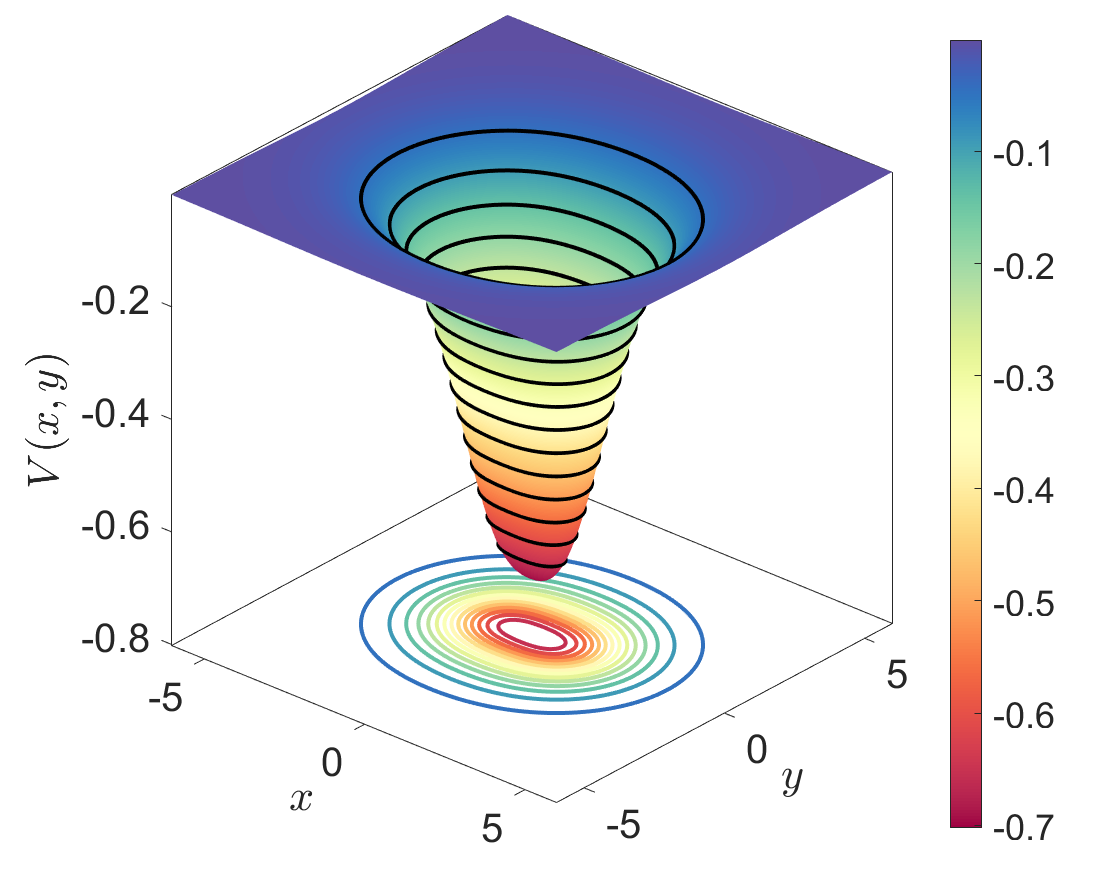
\includegraphics[scale=0.3]{CirquePES_c_1div2_a_1_b_1div8_d_1.png}
    \caption{Surface plot of Double-vdW potential Equation \eqref{eq:vdw-single}. Parameters used: $C_6 = 1/2$, $\alpha = 1$, $\beta = 1/8$ and $d = 1$}
    \label{fig:vdw-single_surface}
\end{figure}

\begin{figure}[htbp]
    \centering
    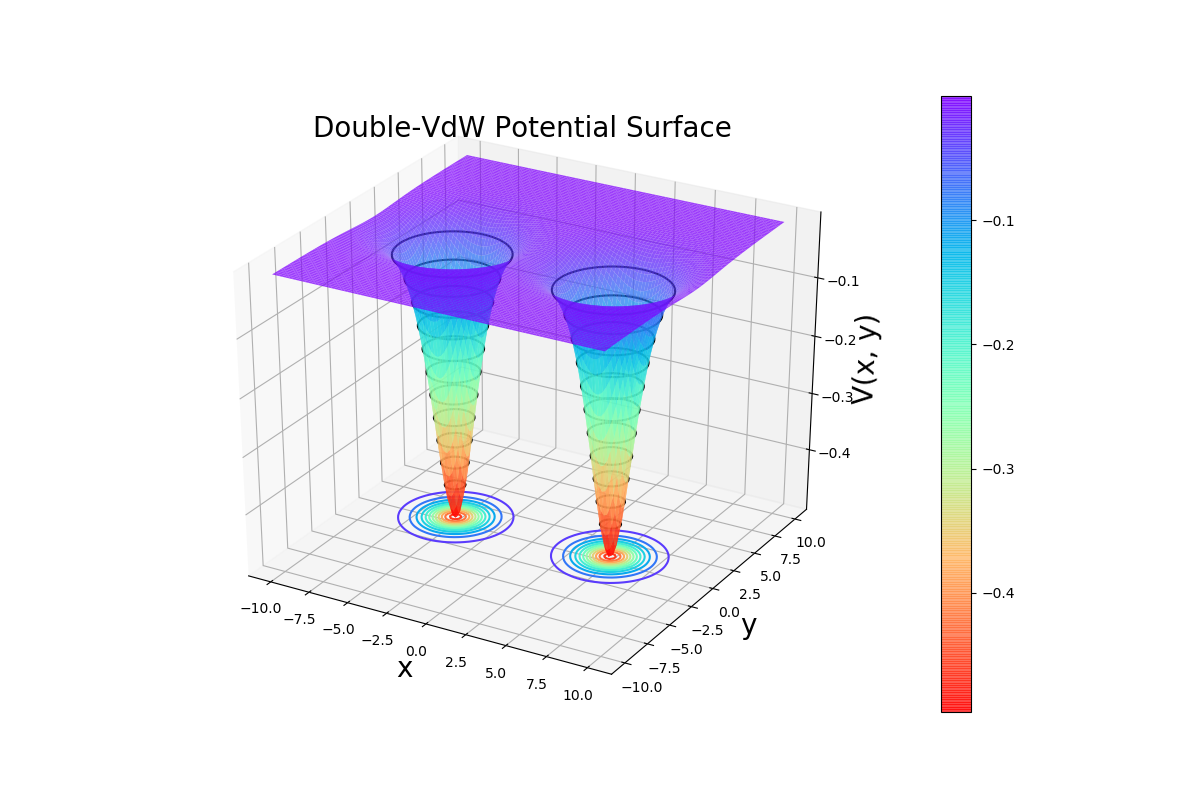
\includegraphics[scale=0.45]{double-vdw_surface.png}
    \caption{Surface plot of Double-vdW potential Equation \eqref{eq:vdw-double}. Parameters used: $C_6 = 1/2$, $\alpha = 1$, $\beta = 1/8$, and  $d = 5$ }
    \label{fig:vdw-double_surface}
\end{figure}

The two degrees-of-freedom Hamiltonian for the Cirque potential energy surface is defined as the classical sum of kinetic plus potential energy:
\begin{equation}
H(x,y,p_x,p_y) = \dfrac{p_x^2}{2 m_1} + \dfrac{p_y^2}{2 m_2} + V(x,y)
\label{eq:hamil}
\end{equation}
Hamilton's equations that determine the systems dynamical evolution are given by:
\begin{equation}
\begin{cases}
\dot{x} = \dfrac{\partial H}{\partial p_x} = \dfrac{p_x}{m_1} \\[.5cm]
\dot{y} = \dfrac{\partial H}{\partial p_y} = \dfrac{p_y}{m_2} \\
\dot{p}_x = - \dfrac{\partial H}{\partial x} = - \dfrac{\partial V}{\partial x} = - 6 \, \beta \, C_6 \left[\dfrac{x - d}{\left(\beta\left[\left(x - d\right)^2 + y^2\right] + \alpha\right)^4} + \dfrac{x + d}{\left(\beta\left[\left(x + d\right)^2 + y^2\right] + \alpha\right)^4}\right] \\[.7cm]
\dot{p}_y = - \dfrac{\partial H}{\partial y} = - \dfrac{\partial V}{\partial y} = - 6 \, \beta \, C_6 \, y \left[\dfrac{1}{\left(\beta\left[\left(x - d\right)^2 + y^2\right] + \alpha\right)^4} + \dfrac{1}{\left(\beta\left[\left(x + d\right)^2 + y^2\right] + \alpha\right)^4}\right]
\end{cases}
\label{eq:ham_eq}
\end{equation}
In this work we will consider the situation where both DoF have unit mass, that is $m_x = m_y = 1$. The equilibrium points $\mathbf{r}_e = (x_e,y_e,p_{x,e},p_{y,e})$ of the dynamical system given above are contained in configuration space, since $p_{x,e} = p_{y,e} = 0$, and they are also critical points of the PES, that is $\nabla V (x_e,y_e) = \mathbf{0}$. It is straightforward to check that under these conditions, the points have to satisfy:
\begin{equation}
y_e = 0 \quad , \quad \left(x_e - d\right) \left[\beta\left(x_e + d\right)^2 + \alpha\right]^4 + \left(x_e + d\right) \left[\beta\left(x_e - d\right)^2 + \alpha\right]^4 = 0 
\label{eq:eq_pts}
\end{equation}
It is straightforward to show that $x_e = 0$ is always a solution to the equation above, and therefore the origin is always an equilibrium point of Hamilton's equations for this system. Moreover, there is also an equilibrium point located at infinity. Regarding the presence of other equilibria, this depends critically on the model parameters, and if they exist, their coordinates are of the form $\mathbf{r}_e = (x_e(\alpha,\beta,d),0,0,0)$. 

The linear stability of these equilibrium points is determined by the eigenvalues of the Jacobian matrix given by the linearization of Eq. \eqref{eq:ham_eq} about each of the points. In order to construct the Jacobian, we need to compute the second order partial derivatives that characterize the Hessian matrix of the PES:
\begin{equation}
\begin{cases}
\dfrac{\partial^{\,	2} V}{\partial x^2} = 6 \, \beta \, C_6 \left[\dfrac{\beta\left[-7\left(x - d\right)^2 + y^2\right] + \alpha}{\left(\beta\left[\left(x - d\right)^2 + y^2\right] + \alpha\right)^5} + \dfrac{\beta\left[-7\left(x + d\right)^2 + y^2\right] + \alpha}{\left(\beta\left[\left(x + d\right)^2 + y^2\right] + \alpha\right)^5} \right] \\[.8cm]

\dfrac{\partial^{\,	2} V}{\partial y^2} = 6 \, \beta \, C_6 \left[\dfrac{\beta\left[\left(x - d\right)^2 - 7 y^2\right] + \alpha}{\left(\beta\left[\left(x - d\right)^2 + y^2\right] + \alpha\right)^5} + \dfrac{\beta\left[\left(x + d\right)^2 - 7y^2\right] + \alpha}{\left(\beta\left[\left(x + d\right)^2 + y^2\right] + \alpha\right)^5} \right] \\[.8cm]

\dfrac{\partial^{\,	2} V}{\partial x \partial y} = - 48 \, \beta^2 \, C_6 \, y \left[\dfrac{x - d}{\left(\beta\left[\left(x - d\right)^2 + y^2\right] + \alpha\right)^5} + \dfrac{x + d}{\left(\beta\left[\left(x + d\right)^2 + y^2\right] + \alpha\right)^5}\right]
\end{cases}
\label{eq:second_pder}
\end{equation}
We take a look now at the Hessian matrix of the PES evaluated at the origin:
\begin{equation}
\text{Hess}_{V}(0,0) = \begin{pmatrix}
\dfrac{\partial^{\,	2} V}{\partial x^2}(0,0) & \dfrac{\partial^{\,	2} V}{\partial x \partial y}(0,0) \\[.4cm]
\dfrac{\partial^{\,	2} V}{\partial y \partial x}(0,0) & \dfrac{\partial^{\,	2} V}{\partial y^2}(0,0)
\end{pmatrix} = \begin{pmatrix}
\dfrac{12 \beta C_6}{\left(\beta d^2 + \alpha\right)^4} \left[1 - \dfrac{8\beta d^2}{\beta d^2 + \alpha}\right] & 0 \\[.5cm]
0 & \dfrac{12 \beta C_6}{\left(\beta d^2 + \alpha\right)^4}
\end{pmatrix}
\end{equation}
The linear stability of the origin is characterized by the nature of the eigenvalues of the Jacobian matrix:
\begin{equation}
J(0,0) = \begin{pmatrix}
\mathbb{O}_2 & \mathbb{I}_2 \\[.3cm]
-\text{Hess}_{V}(0,0) & \mathbb{O}_2
\end{pmatrix} = \begin{pmatrix}
0 & 0 & \hspace{.2cm} 1 & \hspace{.5cm} 0 \hspace{.2cm} \\[.4cm]
0 & 0 & \hspace{.2cm} 0 & \hspace{.5cm} 1 \hspace{.2cm} \\[.4cm]
\dfrac{12 \beta C_6}{\left(\beta d^2 + \alpha\right)^4} \left[\dfrac{8\beta d^2}{\beta d^2 + \alpha} - 1\right] & 0 & \hspace{.2cm} 0 & \hspace{.5cm} 0 \hspace{.2cm} \\[.4cm]
0 & -\dfrac{12 \beta C_6}{\left(\beta d^2 + \alpha\right)^4} & \hspace{.2cm} 0 & \hspace{.5cm} 0 \hspace{.2cm} 
\end{pmatrix}
\end{equation}
The eigenvalues $\xi$ are given by:
\begin{equation}
\xi_{1,2} = \pm \, \omega \, i \quad,\quad \xi_{3,4} = \pm \, \omega \, \sqrt{\dfrac{8\beta d^2}{\beta d^2 + \alpha} - 1}
\end{equation}
where we have that:
\begin{equation}
\omega = \dfrac{2 \sqrt{3\beta C_6}}{\left(\beta d^2 + \alpha\right)^2}
\end{equation}
is the angular frequency of oscillation in the linear approximation. Therefore, the origin is an index-1 saddle equilibrium point when the condition $7\beta d^2 \geq \alpha$ is met. However, for $7\beta d^2 < \alpha$ it turns out into a potential well (a center equilibrium point). This indicates that there is a pitchfork bifurcation taking place in the PES at the origin at the critical relation $7\beta d^2 = \alpha$. We illustrate this behavior below by looking at the value of the potential along the $x$-axis:

\begin{figure}
    \centering
    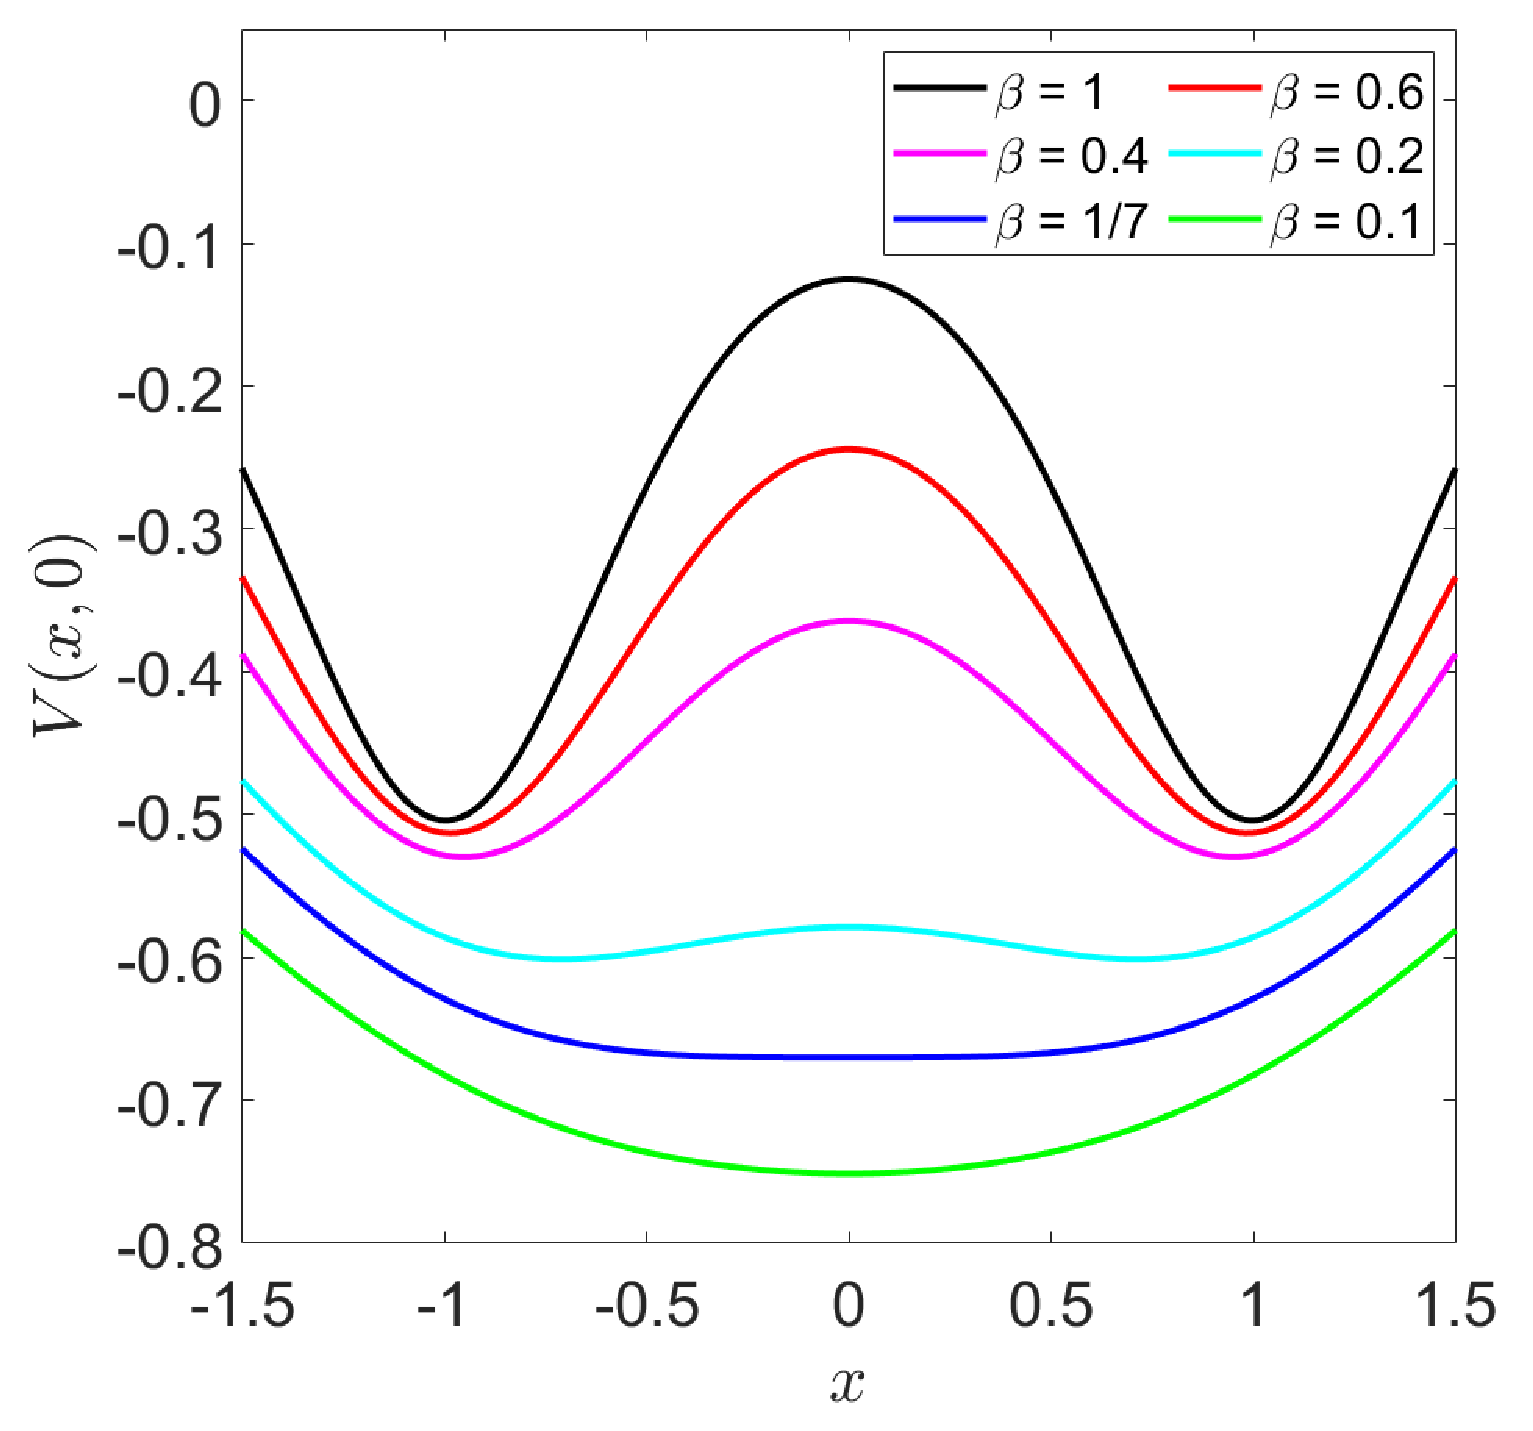
\includegraphics[scale=0.36]{pitcfork_bif_c_1div2_a_1_d_1}
    \caption{}
    \label{fig:pitchfork_bif}
\end{figure}


\bibliography{cirque}

\end{document}
